In diesem Kapitel werden das E- und B-Feld betrachtet.
Des Weiteren wird ihre Wechselwirkung betrachtet.
In diesem Kapitel wird für das E-Feld die Quelle \cite{Animation}.
Im Abschnitt zum B-Feld wird die Quelle \cite{Lorentzkraft}verwendet.
%\section{E-Feld}
%\subsection{Entstehung und Beschreibung}
\section{Entstehung und Beschreibung des E-Feldes}
Jede Ladung wird von einem elektrischen Feld umgeben.
Zuerst muss der Begriff von Ladung geklärt werden:
Ladung ist eine Eigenschaft von Materie.
Die Einheit der Ladung ist $1C$ (Coulomb).
Alle bisherigen Experimente legen nahe, dass es nur 2 Arten von elektrischer Ladung gibt; Positiv und Negativ.
Eine Ladung bewirkt eine Kraft auf eine andere Ladung.
Gleich geladene Ladungen stoßen sich ab, während entgegengesetzt geladene Ladungen sich anziehen.
Diese Kraft wird als elektrische Kraft bezeichnet oder genauer als Coulomb-Kraft.
Die Richtung der Feldlinien ist immer die Richtung der Kraftwirkung auf einen positiv geladenen Probekörper.
Der experimentelle Nachweis der Coulomb-Kraft sieht wie folgt aus:
Man nehme sich zwei Punktladungen, welche mit $q_1$ und $q_2$ bezeichnet werden. 
Des Weiteren ist ein Abstand $r$ zwischen den Ladungen vorhanden.
Es gibt einmal die Kraft von $q_1$ auf $q_2$ ($\vv{F_{12}}$) und einmal die Kraft von $q_2$ auf $q_1$ ($\vv{F_{21}}$).
\begin{equation*}
%\label{eq:F_el}
   F_{el} = \frac{1}{4 \cdot \pi \cdot \epsilon_r} \cdot \frac{q_1 \cdot q_2}{r^2}    
\end{equation*}
Dabei stellt $\epsilon_r$ eine Materialeigenschaft dar.
Durch Betrachten der obigen Formel lässt sich schließen, dass wenn $r$ gleich bleibt, aber die Ladungen $q_1$ und $q_2$ erhöht werden, die Coulomb-Kraft ebenfalls zunimmt.
Daraus lässt sich schließen, dass die elektrische Kraft proportional zu den Ladungen $q_1$ und $q_2$ ist. 
Wenn die Ladungen $q_1$ und $q_2$ gleich bleiben und $r$ erhöht wird, dann verringert sich die elektrische Kraft.
Daraus lässt sich wiederum schließen, dass die elektrische Kraft quadratisch anti-proportional zum Abstand $r$ ist.
Diese zuvor beschriebene Kraftwirkung, lässt sich mittels Probeladungen im ganzen Raum um die Ladung messen und als Vektor an jedem Punkt visualisieren.
Diese Visualisierung des Raumes nennt man elektrisches Feld.
Die jeweilige Stärke ergibt sich aus der Größe der Probeladung $q$ und der Größe der Kraft $F_{el}$ auf die Ladung.
Die Formel für das E-Feld ist:
\begin{equation*}
%\label{eq:E}
    E = \frac{F_{el}}{q}
\end{equation*}
Die Dimension des E-Feldes lautet: $[E] = \frac{N}{C} = \frac{V}{m}$.
Veranschaulichen lässt sich die Coulombkraft durch die Animation \cite{Animation}.

%Beschreibung
Wenn ein elektrisches Feld vorhanden ist, lässt sich dieses als Eigenschaft des Raums auffassen.
Die Kraftwirkung des elektrischen Feldes wird mit Probeladung ermittelt und durch Feldlinien visuell dargestellt.
Die Feldlinien kreuzen und berühren sich nicht.
Wenn die Feldlinien eng beieinander liegen (hohe Dichte), dann ist das dort existierende elektrische Feld stark.
Wenn die Dichte der Feldlinien allerdings niedrig ist, dann ist das elektrische Feld schwach.
Es gibt zwei unterschiedliche Arten von elektrischen Feldern. 
Es gibt zum einen das homogene elektrische Feld und zum anderen das inhomogene elektrische Feld.
Bei dem homogenen elektrischen Feld stehen die Feldlinien parallel zu einander und das elektrische Feld ist an allen Stellen gleich stark.
Bei dem inhomogenen elektrischen Feld kann diese Annahme nicht getätigt werden.
% hier eventuell noch auf die verschiedene Ladungen eingehen (Punktladung, etc.)
%\subsection{Anwendung}
\section{Anwendung des E-Feldes}
\label{sec:Plattenkondensator}
Als Anwendungsbeispiel lässt sich der Plattenkondensator nehmen:
Hier lässt sich die Annahme treffen, dass das elektrische Feld zwischen den Platten homogen ist.
Allerdings muss beachtet werden, dass diese Aussage nur zwischen den Platten des Kondensators gilt, und sobald man an die Ränder des Kondensators geht, diese Aussage wegbricht.
An den Rändern wirkt nämlich ein inhomogenes elektrisches Feld.
Des Weiteren ist das elektrische Feld als $E = \frac{U}{d}$ zu bestimmen.
Somit nimmt das elektrische Feld bei einer größeren Spannung $U$ zu und bei größerem Abstand $d$ der Platten ab.
Beim Kondensator kann noch eine weitere Größe eingeführt werden, die Kapazität $C$.
Die Kapazität ist dabei so definiert, dass sie die maximale Menge an Ladung angibt, die der Kondensator auf den Platten speichern kann.
Die Herleitung ist wie folgt:
$\mbox{Flächenladungsdichte} \sigma \mbox{=} \frac{Q}{A}$.
Dies führt zum elektrischen Feld mit $\sigma = \epsilon_0 \cdot E$ als Feldgleichung.
Dabei beträgt $\epsilon_0 = 8.854 \cdot 10^{-12} \frac{As}{Vm}$ und ist unter dem Namen "`Dielektrizitätskonstante"' bekannt.
Im Allgemeinen ist das Feld auch noch vom jeweiligen Material abhängig, wodurch die Gleichung einen weiteren Term $\epsilon_r$ enthält: $\sigma = \epsilon_0 \cdot \epsilon_r \cdot E$.
Diese zusätzliche Konstante berücksichtigt dabei die spezifischen Materialeigenschaften und nennt sich "`relative Permeabilität"'.
Im Vakuum ist diese jedoch = 1.
Daraus folgt, dass $ Q = \epsilon_0 \cdot \epsilon_r \cdot \frac{A}{d} \cdot U$ ist.
Die Kapazität ist dann als
\begin{equation*}
%\label{eq:C}
    C = \frac{Q}{U} = \epsilon_0 \cdot \epsilon_r \cdot \frac{A}{d}
\end{equation*}
definiert.
%\section{B-Feld:}
%\subsection{Entstehung und Beschreibung}
\section{Entstehung und Beschreibung des B-Feldes}
Beim Nähern von 2 Magneten wurde festgestellt, dass sich gleiche Pole abstoßen und ungleiche anziehen.
Diese Kraftwirkung wurde historisch als die Magnetische Feldstärke $H$ definiert.
Das ist die eigentliche Entsprechung zum E-Feld.
Da es in der Anwendung einfacher ist, wird im Folgenden mit dem Magnetfeld das B-Feld gemeint.\footnote{In der Quelle \cite{Gente1950} wird mit der Formel $\mu_0 \cdot H$ gerechnet, während bei den verwendeten Formeln im Kapitel \ref{sec:a} mit $B$ gerechnet wird.}
Der Zusammenhang zwischen $B$ und $H$ ist wie folgt: $B = \mu_r \cdot \mu_0 \cdot H$.
Dabei ist die Dimension von $H$ : $[H] = \frac{A}{m}$.
Als Grundlage, dass ein B-Feld entsteht, muss der Magnetismus genommen werden.
Dafür muss der Begriff des Magnetismus zuerst geklärt werden.
Ein Magnet wird dadurch entmagnetisiert, dass er gestoßen oder auf einer Temperatur oberhalb der Curie-Temperatur erhitzt wird $ \approx 600 ~ ^\circ C$.
Des Weiteren führt das Durchbrechen eines Stab-Magneten in der Mitte dazu, dass zwei neue Magnete entstehen, es gibt also keine magnetischen Monopole.
Die Feldlinien eines Magneten verlaufen vom Nordpol zum Südpol.
Ein Magnetfeld bewirkt eine Kraft auf ein bewegtes geladenes Teilchen.
Die wirkende Kraft wird als magnetische Kraft bezeichnet oder als Lorentzkraft, wenn es sich um einen einzelnen Ladungsträger handelt.
Die Herleitung der Lorentzkraft sieht wie folgt aus:
Man nehme sich einen Ladungsträger (negativ) und einen langen Leiter.
Die Formel für die magnetische Kraft lautet: $F_{mag} =  B \cdot I_L \cdot \Delta l$.
Der Strom $I_L$ kann durch $\frac{\Delta Q}{\Delta t}$ ersetzt werden.
Dadurch kommt die Formel $F_{mag} = B \cdot \frac{\Delta Q}{\Delta t} \cdot \Delta l$ heraus.
Als nächstes lässt sich $\Delta Q$ durch $N \cdot e$ ersetzen.
Dabei stellt $N$ die Menge an Elektronen dar, welche betrachtet werden.
Dies führt zu der Formel $F_{mag} = B \cdot N \cdot e \cdot \frac{\Delta l}{\Delta t}$.
Dabei lässt sich der Quotient als $v$ vereinfachen, was die Geschwindigkeit der Ladungsträger angibt.
Dadurch beträgt die Formel für die magnetische Kraft nun: $F_{mag} = B \cdot N \cdot e \cdot v$.
Allerdings soll die Lorentzkraft hergeleitet werden, welche die Kraft auf einen einzelnen Ladungsträger darstellt, weshalb die magnetische Kraft mit $N$ dividiert werden muss.
Dies führt dazu, dass die Formel für die Lorentzkraft $F_L = B \cdot e \cdot v$ ist.
Diese Herleitung lässt sich prinzipiell für jede beliebige Ladung benutzen, weshalb $e$ durch $q$ ersetzt werden kann.
Daraus ergibt sich die Formel:
\begin{equation*}
%\label{eq:F_l1}
    F_L = q \cdot B \cdot v
\end{equation*}
Hier wird angenommen, dass der Geschwindigkeitsvektor senkrecht auf dem Vektor der Flussdichte steht.
Ist dies nicht der Fall, kann die Formel mit $\sin(\alpha)$ multipliziert werden, wobei $\alpha$ den Winkel zwischen den beiden Vektoren darstellt.
Der Vektor der Lorentzkraft steht senkrecht auf der durch den Geschwindigkeitsvektor und den Vektor der Flussdichte aufgespannten Ebene \cite{Lorentzkraft}.

Magnetfelder entstehen in der Gegenwart von Dauermagneten (bestehend aus Eisen, Kobalt, Nickel oder deren Legierungen) oder in der Umgebung von stromdurchflossenen Leitern. 
Die Größe der magnetischen Flussdichte $B$ ist den magnetischen Feldlinien zugeordnet.
Sie ist durch die Kraft definiert, welche ein stromdurchflossener Leiter erfährt.
Die Visualisierung des Raums, in welchem das Magnetfeld wirkt, nennt man magnetisches Feld.
Die jeweilige Stärke ergibt sich aus der Größe der Kraft $F_L$, der Länge des Leiters $l$ und der Stärke des elektrischen Stroms $I$.
Die Formel für das B-Feld ist:
\begin{equation*}
%\label{eq:B}
    B = \frac{F_L}{I \cdot l}
\end{equation*}
Die Dimension des B-Feldes lautet: $[B] = \frac{N}{Am} = \frac{Vs}{m^2} = T$.
Dabei steht $T$ für Tesla und stellt die Einheit für die Stärke des Magnetfeldes dar.

% Beschreibung von B-Feld
Wenn ein magnetisches Feld vorhanden ist, lässt sich dieses als Eigenschaft des Raums auffassen.
Die Feldlinien kreuzen und berühren sich nicht.
Des Weiteren haben Sie keinen Anfangspunkt und keinen Endpunkt, sondern sind stets geschlossen.
Wenn die Dichte an Feldlinien groß ist, dann ist die Magnetfeldstärke dementsprechend ebenfalls stark.
Wenn die Dichte an Feldlinien gering ist, dann ist die Magnetfeldstärke ebenfalls gering.
Es gibt verschiedene Magnete mit dementsprechend auch verschiedenen Formen von Magnetfeldern. 
Zum einen liegt der Stabmagnet vor, bei welchem das magnetische Feld analog zum elektrischen Feld eines Dipols ist.
Zum anderen liegt der Hufeisenmagnet vor, bei welchem im Inneren das Feld gleich wie das elektrische Feld beim Plattenkondensator aussieht.
Bei diesem ist also das magnetische Feld im Inneren homogen, allerdings an den Rändern inhomogen. 
%\subsection{Anwendung}
\section{Anwendung des B-Feldes}
\label{sec:Fadenstrahlrohr}
Als Anwendungsbeispiel lässt sich das Fadenstrahlrohr nehmen.
Hier lässt sich die Annahme treffen, dass das magnetische Feld im Inneren einer Helmholtz-Spule homogen ist. Des Weiteren gelangen die betrachteten Elektronen mit einer Geschwindigkeit von 
\begin{equation}
\label{eq:v1}
    v=\sqrt{\frac{2 \cdot e \cdot U_B}{m}}
\end{equation}
in die Helmholtz-Spule.\footnote{Diese Formel wird weiter hinten in der Arbeit hergeleitet, siehe Formel (\ref{eq:v}) dort.}
Die Elektronen wurden davor in einer Elektronenkanone freigesetzt.
Dies ist in Kapitel \ref{sec:tolle-section} dargestellt. 
Das Fadenstrahlrohr kann verwendet werden, um die spezifische Ladung $\frac{e}{m}$ eines Elektrons oder eines Ions zu bestimmen.
Dafür kann man durch die Linke-Hand-Regel die Richtung der Ablenkung eines einzelnes Elektrons im Magnetfeld bestimmen.
Dabei zeigt der Daumen die Richtung der Geschwindigkeit der negativen Ladungsträger an, der Zeigefinger die Richtung der Feldlinien und der Mittelfinger die senkrecht dazu wirkende Lorentzkraft.
Wenn nun also ein Elektron senkrecht zu den Feldlinien in ein Magnetfeld eintritt, kommt man zu dem Schluss, dass die Elektronen auf einer Kreisbahn abgelenkt werden. 
Dadurch wirkt die Lorentzkraft als Zentripetalkraft und es kann gleichgesetzt werden:
$$F_L = F_z$$
$$e \cdot v \cdot B = \frac{m \cdot v^2}{r}$$
Einsetzen von (\ref{eq:v1}) und  Umformen nach $\frac{e}{m}$ ergeben die folgende Formel.
\begin{equation*}
%\label{eq:e/m}
    \frac{e}{m} = \frac{2 \cdot U_B}{ r^2 \cdot B^2}
\end{equation*}
Diese Formel gibt die spezifische Ladung eines Elektrons an, allerdings kann man $e$ auch durch $q$ ersetzen und dadurch die spezifische Ladung eines jeden anderen Ions bestimmen, indem der jeweilige Radius beobachtet wird.
\section{Wechselwirkung der Felder}%Maxwellgleichung
\label{sec:Maxwell}
Der folgende Abschnitt bezieht sich hauptsächlich auf die Quelle \cite{Maxwell}.

Mit der Wechselwirkung zwischen den Feldern hat James Clerk Maxwell sich
beschäftigt.
Maxwell arbeitete von 1861 bis 1864 an den Gleichungen.
Er leitete die sogenannten "`Maxwell-Gleichungen"' her, welche die Zusammenhänge zwischen elektrischen und magnetischen Feldern untereinander und den Zusammenhang mit elektrischem Strom und elektrischer Ladung beschreiben.
Wenn die Lorentzkraft noch dazu genommen wird, dann kann die gesamte klassische Elektrodynamik erklärt werden.

Als erstes wird die Wechselwirkung von statischen Feldern betrachtet.
Dabei sind die elektrischen und magnetischen Felder konstant und überlagern sich ungestört.
Dabei gilt für die Kraft die Formel: $F_{Ges} = Q (E + v \times B)$.
Hier ist sowohl die elektrische als auch die Lorentzkraft wiederzufinden.
Die Lorentzkraft ergibt sich, wenn die Stärke des elektrischen Feldes $E$ gleich null ist.
Die Formel der elektrischen Kraft hingegen entsteht, wenn die Geschwindigkeit $v$ gleich null ist.
%Denn auf bewegte Teilchen wirkt die Lorentzkraft und nicht aber die elektrische Kraft.
Es gibt keine gegenseitige Beeinflussung der Felder, wenn sie stationär sind. 
Die Beeinflussung tritt erst bei sich zeitlich verändernden Feldern auf.
Dies lässt sich mit Hilfe der sogenannten "`Maxwell-Gleichungen"' betrachten.
Diese wären:
\begin{equation}
\label{eq:div E}
    \nabla \cdot E = \frac{1}{\epsilon_o} \cdot \rho
\end{equation}
\begin{equation}
\label{eq: div B}
    \nabla \cdot B = 0
\end{equation}
\begin{equation}
\label{eq:rot E}
    \nabla \times E = - \frac{\partial B}{\partial t}
\end{equation}
\begin{equation}
\label{eq:rot B}
    \nabla \times B = \mu_0 \cdot j + \mu_0 \cdot \epsilon_0 \cdot \frac{\partial E}{\partial t}
\end{equation}
Für die Wechselwirkung zwischen elektrischen und magnetischen Feldern ist nur die Betrachtung der Gleichungen (\ref{eq:rot E}) und (\ref{eq:rot B}) notwendig.
Die ersten beiden Gleichungen dienen hier als wichtige Grundlage und beschreiben das Entstehen der beiden Felder.
Die Maxwell-Gleichungen sind wie folgt zu lesen: 
Das "`$ \nabla \cdot$"' bedeutet Divergenz und beschreibt die Quelle des E-Feldes.
Wie die rechte Seite der Gleichung (\ref{eq:div E}) zeigt, ist diese Quelle die Ladungsdichte $\rho$.
Dies bedeutet, dass die Gleichung (\ref{eq:div E}) zeigt, dass die Quelle für das E-Feld die Ladung ist.
Die Gleichung (\ref{eq: div B}) zeigt, dass das B-Feld keine Quelle hat, da es ohne Quellen keine Monopole geben kann, aus welchen das B-Feld entspringt.
Ebenso begründet diese Gleichung den stets geschlossenen Verlauf der magnetischen Feldlinie, da es keinen Anfang gibt.
Dies lässt sich am Beispiel des Stabmagneten zeigen.
Dort verlassen die Feldlinien den Magneten am Nordpol und treten am Südpol wieder ein.
Auch im Inneren laufen diese Feldlinien weiter in Richtung des Nordpols und bilden so eine geschlossene Bahn ohne Anfang und ohne Ende.
Dies ist in der Abbildung \ref{fig:stabm} zu sehen.

\begin{figure}[h]
    \centering
    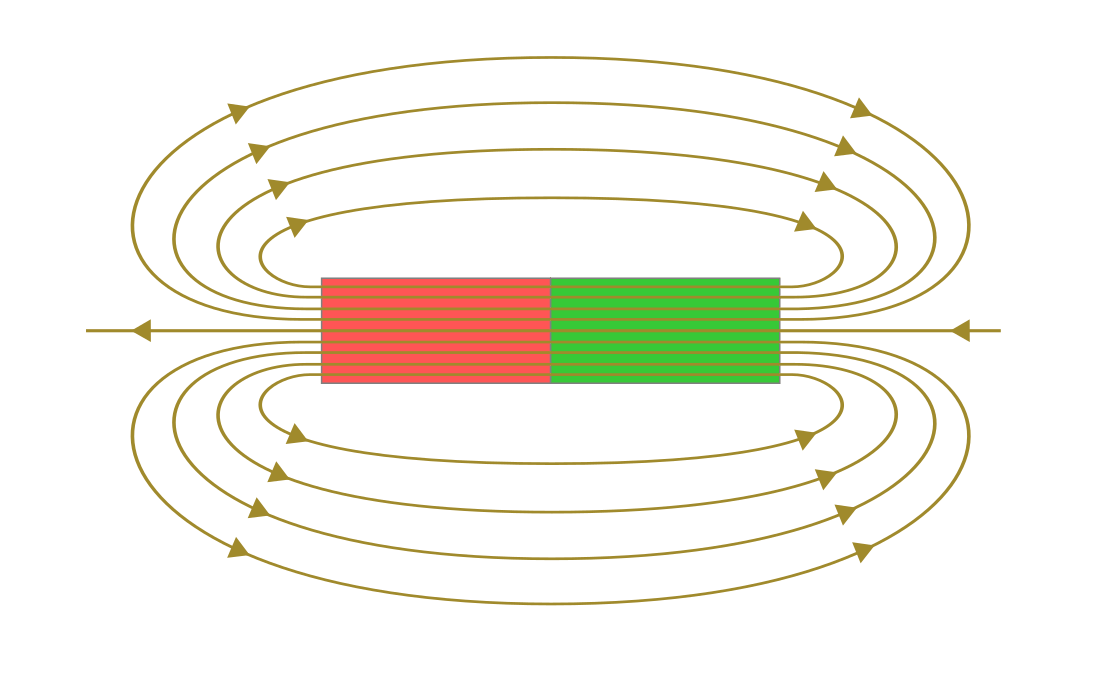
\includegraphics[width=.9\textwidth]{fig/feldlinien-stabmagnet (1).png}
    \caption{Feldlinien eines Stabmagneten (übernommen von \cite{Stabmagnet})}
    \label{fig:stabm}
\end{figure}
Die Gleichung (\ref{eq:rot E}) zeigt, dass ein entgegengesetztes sich zeitlich änderndes magnetisches Feld ein sich rotierendes elektrisches Feld erzeugt.
Das "`$ \nabla \times$"' ("`$\times$"' steht für das Kreuzprodukt) bedeutet Rotation und beschreibt die Rotation des Feldes.
Das Minus in der Gleichung und die Erklärung, dass ein entgegengesetztes magnetisches Feld entsteht, lässt sich mit Hilfe der Lentzschen Regel begründen.
Diese behauptet, dass der Induktionsstrom stets so gerichtet ist, dass er der Ursache seiner Entstehung entgegenwirkt.
Die Gleichung (\ref{eq:rot B}) zeigt, dass eine Spannung (Verschiebungsstrom) und ein sich zeitlich änderndes elektrisches Feld ein rotierendes magnetisches Feld erzeugen.
Die Formeln zeigen, dass die Wechselwirkung zwischen den Feldern ein beständiger Kreis ist. 
Ein sich veränderndes elektrisches Feld erzeugt somit ein magnetisches Feld, welches auch wiederum ein elektrisches Feld erzeugt.
Diese gegenseitige Wechselwirkung setzt sich zeitlich fort, sodass weitere Felder erzeugt werden.
Dieser Kreislauf läuft beständig weiter.

